\section{Problema 3: Girls Scouts}
\subsection{Descripción de la problemática}

En este ejercicio existe un grupo de niñas exploradoras, algunas de ellas amigas entre sí, que deben formarse en una ronda. Siendo $e$ la cantidad de exploradoras, existen $(e-1)!$ permutaciones posibles en las cuales pueden sentarse. Podemos medir la distancia entre dos amigas como la mínima cantidad de chicas que hay entre una y otra, más 1. Por ejemplo, si una chica está al lado de la otra, la distancia entre ellas es 1. Si tenemos una ronda de tres chicas, la distancia entre cualquier par de chicas va a ser 1.

El problema consiste en hallar la forma de ubicar a las exploradoras de forma tal que exista la menor distancia posible entre cada amistad, y logrando que la suma total de la distancia entre todos los pares de amigas sea mínima.

El formato de entrada es un archivo de texto que contiene una línea por cada grupo de exploradoras. Cada línea se compone de una sucesión de amistades separadas por \texttt{;} de la forma \texttt{amistad[;amistad]}. Cada amistad es un par \texttt{x xs} donde \texttt{x} es una letra y \texttt{xs} una cadena de letras.

Veamos un ejemplo. Tenemos un grupo de 5 chicas: A, B, C, D y E. A es amiga de B y C, y D es amiga de C. Esto se puede escribir de muchas maneras. Si escribimos a cada amistad dos veces, podemos hacerlo así:

\texttt{A BC;B A;C AD;D C;E}

Si las sentamos así:

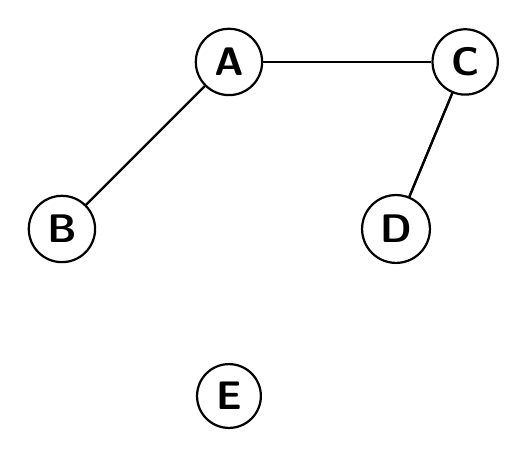
\begin{tikzpicture}[auto, node distance=3cm, every loop/.style={},
                    thick,main node/.style={circle,draw,font=\sffamily\Large\bfseries}]

  \node[main node] (1) {A};
  \node[main node] (2) [below left of=1] {B};
  \node[main node] (3) [below right of=2] {E};
  \node[main node] (4) [below right of=1] {D};
  \node[main node] (5) [right of=1] {C};

  \path[every node/.style={font=\sffamily\small}]
    (1) edge node [left] {} (2)
        edge node[right] {} (5)
    (2) edge node [right] {} (1)
    (4) edge node [left] {} (5)
    (5) edge node {} (4);
\end{tikzpicture}

vamos a estar obteniendo una solución óptima, ya que la suma total de distancias es 3 (contando a cada amistad una sola vez) y la distancia máxima es 1.

El formato de salida para cada grupo de exploradoras es una línea de texto donde se debe indicar la distancia máxima obtenida, seguida de un espacio y una cadena de letras que indica la forma en que fueron sentadas las exploradoras. En caso de haber obtenido más de una solución, se debe devolver la primera en órden alfabético. Para el último ejemplo, la forma de codificar sería así:

\texttt{1 ACDEB}

Nótese que es equivalente a esta otra: \texttt{1 CDEBA}, ya que la única diferencia es por cuál exploradora empezamos a describir la ronda.

%El algoritmo a implementar debe hallar, utilizando backtracking, la permutación en donde la separación entre las niñas que son amigas sea mínima. La técnica algorítmica para resolver el problema puede reducirse a una decisión simple en cada paso: para cada posicion, determinar a qué niña colocar. La mecánica del backtracking busca detectar las instancias en donde los resultados serán peores que el mejor caso registrado, independientemente de las decisiones que se tomen adelante en esa misma rama; de esta forma, se evita el computo de permutaciones que no resultarán óptimas.


\subsection{Algoritmo desarrollado}

Desarrollamos un algoritmo que utiliza la técnica de \textit{backtracking}. Esta técnica consiste en generar de forma incremental candidatos parciales para formar soluciones, haciéndolo de manera tal de poder, en cada paso, evaluar si completar la solución parcial puede resultar en una solución válida o no. De esta manera, si se decide que no se pueden generar soluciones válidas a partir del candidato parcial, se puede abandonar la generación de todas las soluciones que derivan de éste.



La mecánica del algoritmo recursivo consiste en encontrar la mejor permutación posible desde determinada posición (dejando fijos los i primeros elementos).
Para esto, el algoritmo fija un valor en la posición i-esima y se llama recursivamente. Al volver de la recursion, se cambia el valor en la posición i-esima y se vuelve a llamar a la recursion, hasta que se hayan probado todos los valores posibles.
Cuando se detecta una instancia mejor a la anterior, se guarda una copia de la misma, y se recupera posteriormente si no se ha detectado un mejor caso.

\subsection{Justificación de correctitud}

\subsection{Análisis de la complejidad temporal}
La cantidad de posibles permutaciones para una ronda es de '(e-1)!'; en el peor escenario posible, los datos de entradas tienen un orden tal que el algoritmo encuentre una mejor situación en cada iteración, por lo cual tendrá que recorrer las '(e-1)!' permutaciones. 

En cada colocación de una exploradora, se deberá calcular que distancia existe entre ella y sus amigas, lo cual en un peor caso tiene un costo de O(a ln a)
Entonces, en el peor caso, la complejidad del algoritmo pertenece a $O( (e-1)! e a ln a), == O( (e)! a ln a)$,   lo cual es menor que $O(ee a lna) (e! < e^e)$, menor a  $O(ee a2) (a ln a < a^2)$

\subsection{Tests de correctitud}

\subsection{Experimentación para observar la performance real}

\subsubsection{Peor caso}

\subsubsection{Caso promedio}
